\begin{frame}{Thực nghiệm - Phân loại cấu hình}
  \begin{figure}
    \centering
    \subfloat[Lớp C]{
\includegraphics[width=0.3\linewidth]{figures/cls_c.png}}\quad
    \subfloat[Lớp R]{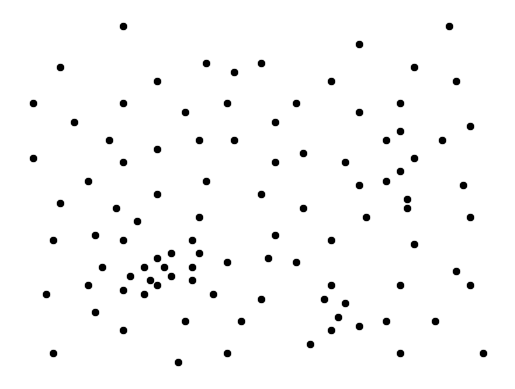
\includegraphics[width=0.3\linewidth]{figures/cls_r.png}}\quad
    \subfloat[Lớp RC]{
\includegraphics[width=0.3\linewidth]{figures/cls_rc.png}}
  \caption{Lớp các cấu hình}
  \label{fig:perf_ct_c1}
  \end{figure}
\end{frame}

\begin{frame}{Thực nghiệm - Phân loại cấu hình}
  \begin{figure}
    \centering
    \subfloat[Lớp C]{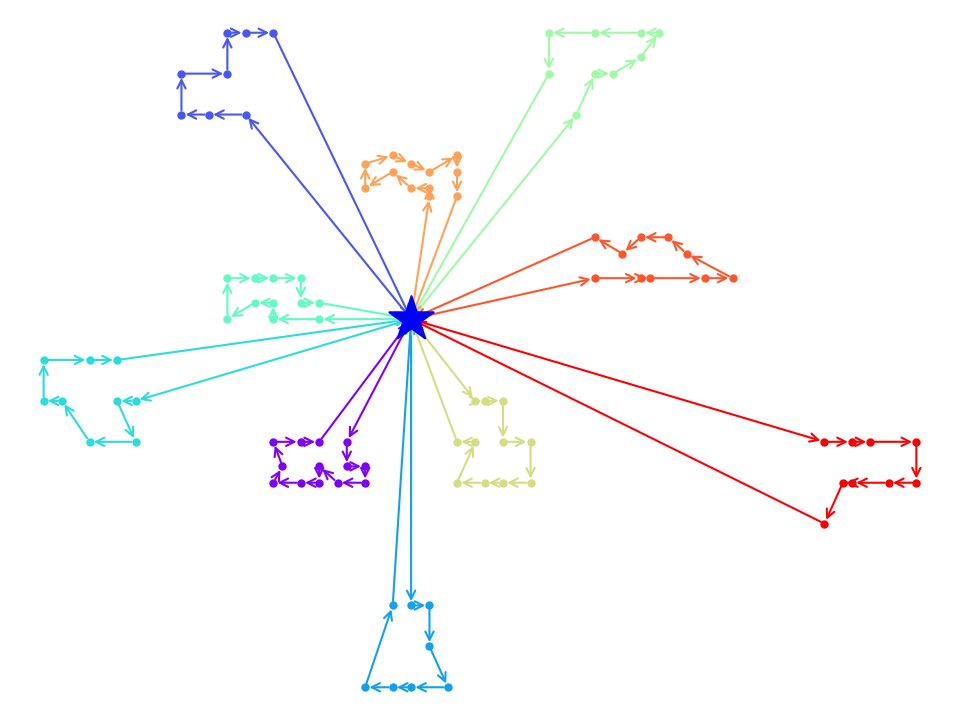
\includegraphics[width=0.3\linewidth]{figures/routes_c101.png}}\quad
    \subfloat[Lớp R]{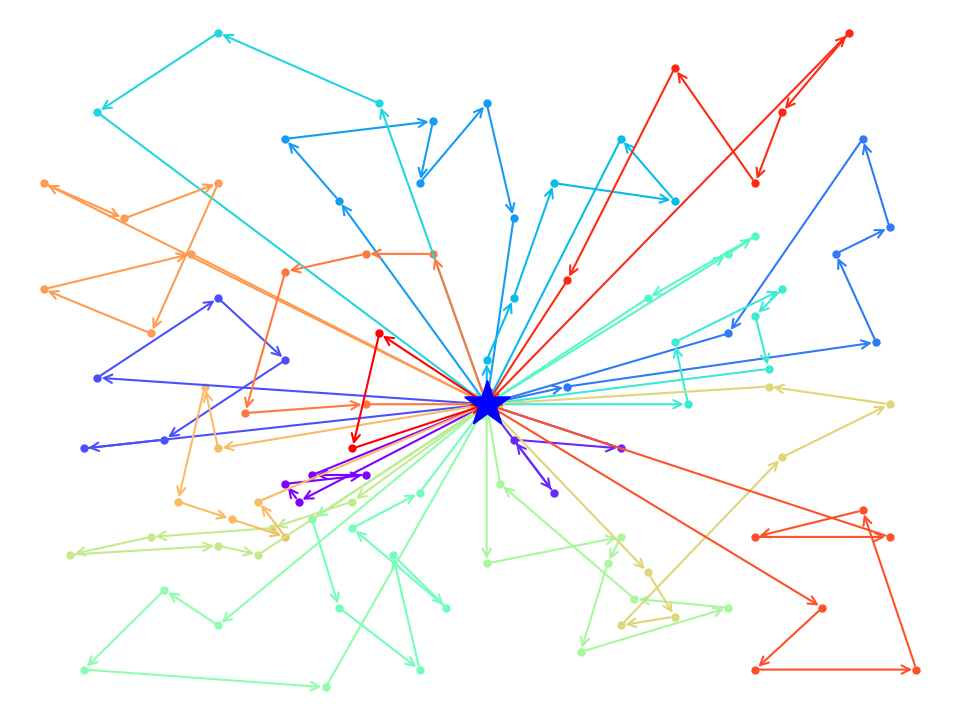
\includegraphics[width=0.3\linewidth]{figures/routes_r101.png}}\quad
    \subfloat[Lớp RC]{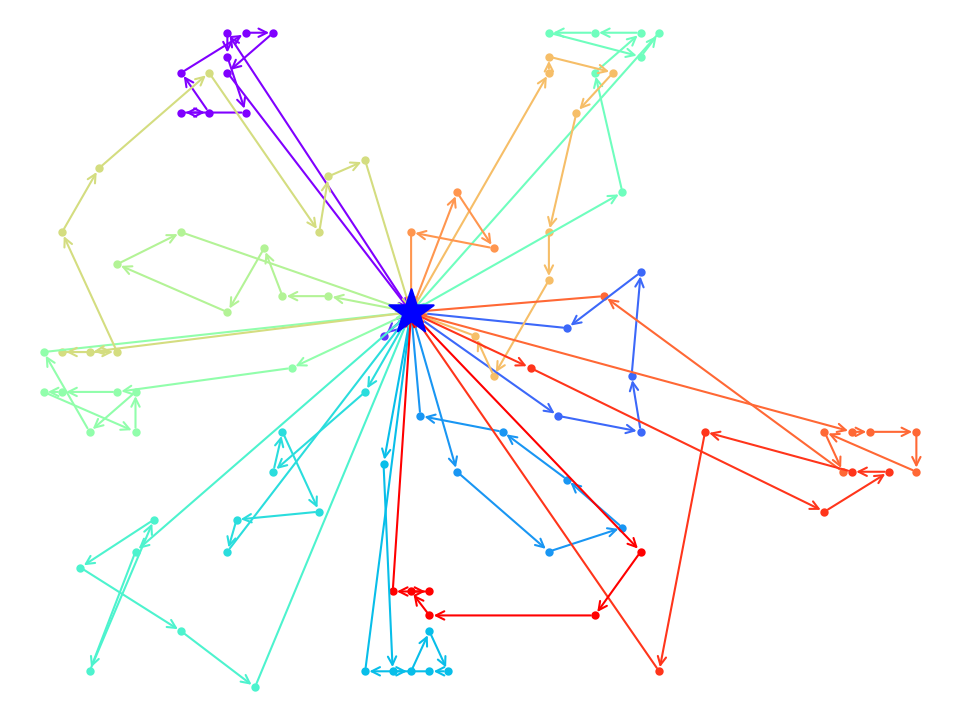
\includegraphics[width=0.3\linewidth]{figures/routes_rc101.png}}
    \caption{Minh họa lời giải cho các lớp cấu hình}
  \end{figure}
\end{frame}

\begin{frame}{Thực nghiệm}
  \begin{block}{Định dạng cấu hình Solomon}
    \begin{itemize}
      \item Tên cấu hình
      \item Số xe được sử dụng
      \item Tải trọng của mỗi xe
      \item ID của yêu cầu
      \item Tọa độ các yêu cầu
      \item Nhu cầu (về tải) của mỗi yêu cầu
      \item Khung thời gian của mỗi yêu cầu
      \item Thời gian phục vụ của mỗi yêu cầu
    \end{itemize}
  \end{block}
\end{frame}

\begin{frame}{Thực nghiệm - Tập Solomon}
  
\end{frame}